%===============================================================================
% zentrale Layout-Angaben und Befehle
%===============================================================================
%
% fr bessere Sicht von falschen Umbrchen die Option draft benutzen
% dadurch knnen aber die eingebundenen Bilder nicht sichtbar sein 
\documentclass[a4paper, 12pt]{article}
%
% hier zun�hst die bentigten packages
\usepackage[english]{babel}
\usepackage[latin1]{inputenc}
%\usepackage{fancyhdr}
\usepackage{verbatim}
\usepackage[T1]{fontenc}
\usepackage{ae}
%\usepackage{listings}
\usepackage{color}
%\usepackage{listings}
%\usepackage{bibgerm}
\usepackage{wrapfig}
%
% Einbindung des Grafik-Pakets
%\ifx\pdfoutput\undefined
\usepackage[dvips]{graphicx}
%\else
%\usepackage[pdftex]{graphicx}
%\pdfcompresslevel=9
%\pdfpageheight=297mm
%\pdfpagewidth=210mm
%\fi
%
% Page-Layout
\setlength\headheight{14pt}
\setlength\topmargin{-15,4mm}
\setlength\oddsidemargin{-0,4mm}
\setlength\evensidemargin{-0,4mm}
\setlength\textwidth{160mm}
\setlength\textheight{252mm}
%
% Absatzeinstellungen
\setlength\parindent{0mm}
\setlength\parskip{2ex}
%
% Kopf- und Fusszeile
%\pagestyle{fancy}
%\fancyhf{} % alles lschen
%\fancyhead[LO]{\footnotesize\sc\nouppercase{\leftmark}}
%\fancyhead[RO]{\footnotesize\sc\nouppercase{\rightmark}}
%\fancyfoot[LO]{\footnotesize\sc Distributed and Mobile Systems Group}
%\fancyfoot[RO]{\thepage}
%\renewcommand{\headrulewidth}{0pt}
%\renewcommand{\footrulewidth}{0pt}
%
% bessere Fehlermeldungen
\errorcontextlines=999
%
% Anweisung zur Erstellung der Titelseite
% #1 = Name der Diplomarbeit
% #2 = Autor
% #3 = Abgabedatum
% #4 = Autor
%\renewcommand{\maketitle}[4]

%\end{titlepage}
%}
%
% wird fr Hintergrund von Code bentigt
%\definecolor{hellgrau}{gray}{0.9}
%
% Einstellungen fr Java-Code
%\lstdefinestyle{javaStyle}{%
%  basicstyle=\small,%
%  backgroundcolor=\color{hellgrau},%
%  keywordstyle=\bfseries,%
%  showstringspaces=false,%
%  %language=Java,%
%  %numbers=left,%
%  numberstyle=\tiny,%
%  stepnumber=1,%
%  numbersep=5pt,%
%  extendedchars=true,%
%  xleftmargin=2em,%
%  lineskip=-1pt,%
%  breaklines%
%}
%
% neues environment fr Java-Sourcecode
% #1 = "caption={Hier eigene �erschrift}, label={Hier eigenes Label}"
%\lstnewenvironment{javacode}[1][]{%
%\lstset{style=javaStyle,#1}%
%}{}

\makeatletter
\def\mycounterlabel#1#2{% #1=label, #2=counter
    \begingroup % to keep change to \@currentlabel local
    %\def
    %\@currentlabel{\arabic{#2}}% label := the value of #2
    \label{#1}%
    \endgroup}
\makeatother

%
% Befehl zum Einbinden von Java-Sourcecode aus Datei
% #1 = Dateiname relativ zu src-Verzeichnis
% #2 = �erschrift
% #3 = Label
\newcounter{Listing}
\setcounter{Listing}{0}
\newcommand{\javafile}[3]{
  \refstepcounter{Listing}
  \begin{center}
    \mycounterlabel{#3}{Listing}Listing \theListing: #2 \\
  \end{center}
  \vspace{-1cm}
  \verbatiminput{src/#1}
}
%
% Einbindung eines Bildes
% #1 = label fr \ref-Verweise
% #2 = Name des Bildes ohne Endung relativ zu images-Verzeichnis
% #3 = Beschriftung
% #4 = Breite des Bildes im Dokument in cm
\newcommand{\bildw}[4]{%
  \begin{figure}[htb]%
    \begin{center}%
      \includegraphics[width=#4cm]{images/#2}%
      %\vskip -0.3cm%
      \caption{#3}%
      %\vskip -0,2cm%
      \label{#1}%
    \end{center}%
  \end{figure}%
}

%
% Einbindung eines Bildes mit Seitenbreite
% #1 = label f�r \ref-Verweise
% #2 = Name des Bildes ohne Endung relativ zu images-Verzeichnis
% #3 = Beschriftung
\newcommand{\bild}[3]{%
  \begin{figure}[htb]%
    \centering%
    \includegraphics[width=\textwidth]{images/#2}%
    \vskip -0.3cm%
    \caption{#3}%
    \vskip -0,2cm%
    \label{#1}%
\end{figure}%
}

%
% Umgebung fr Fliesstext um Grafik
% #1 = Ausrichtung: r, l, i, ...
% #2 = Breite des Bildes in cm
% #3 = Name des Bildes ohne Endung relativ zu images-Verzeichnis
% #4 = Beschriftung
% #5 = label fr \ref-Verweise
\newcommand{\fliesstext}[5]{%
\begin{wrapfigure}{#1}{#2cm}%
\includegraphics[width=#2cm]{images/#3}%
\caption{#4}%
\label{#5}%
\end{wrapfigure}%
}
%%% Local Variables: 
%%% mode: latex
%%% TeX-master: t
%%% End: 

\begin{document}
%
% Titelblatt erstellen
%\maketitle{OCoN Framework version 1.0}{Jens Bruhn, 
%jens.bruhn@uni-bamberg.de}{08.06.2004}{Sven Kaffille, 
%sven.kaffille@uni-bamberg.de}%

\begin{titlepage}

\begin{tabular}{ccc}
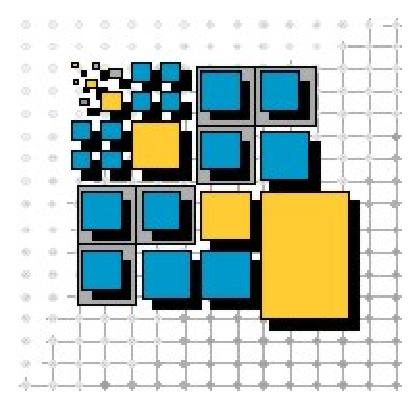
\includegraphics[height=26mm]{include/logo} &

\parbox{11cm}{
  \vspace{-2.6cm}
  \begin{center}
  Otto-Friedrich-Universit\"at Bamberg \newline 
  {\Large Distributed and Mobile Systems Group}
  \end{center}
} &


\includegraphics[height=26mm]{include/uni}\\
\multicolumn{3}{c}{
  \parbox{11cm}{
    \begin{center}
    {\Large
    Open Chord version 1.0.4\\ User's Manual}
    \end{center}
  }
}\\
\end{tabular} 
\\[24pt]
%Vorgelegt von:\\
sven.kaffille@uni-bamberg.de\\
karsten.loesing@uni-bamberg.de\\[18pt]
Lehrstuhl f\"ur Praktische Informatik \\
Otto-Friedrich-Universit\"at Bamberg\\
Feldkirchenstr. 21\\
D-96052 Bamberg\\
GERMANY
\\[12pt]
22.10.2007\\
\newpage

\end{titlepage}

% Erstellung der Inhaltsverzeichnisse
\pagenumbering{Roman}
\tableofcontents
\newpage
\listoffigures
\newpage
%\listoftables
\newpage
\setcounter{page}{1}
\pagenumbering{arabic}
%
% hier einzelne Kapitel mit \input{Kapitel-File} einfgen
\section{What is Open Chord?}
As Peer-to-Peer (P2P) computing becomes more important for distributed applications, 
which have to be reliable, load balanced and scalable, the underlying technologies 
must also provide these properties. 
This is also important for data storage in P2P networks. In recent years new data 
structures -- so-called distributed hash tables (DHT) -- have been shown to provide a 
reliable, load balanced and scalable mechanism to store data in a P2P network. 

DHT differ from P2P networks developed before (e.g. Gnutella) in their structural 
organization. While DHTs are based on structured networks, where for example the nodes 
in the network are organized in a ring, former P2P networks had no structure, which 
ordered the nodes of the networks in a particular way. Therefore these networks could 
not provide guarantees for data stored in the network to be found. The structure of DHTs allows to exactly locate desired data with help of a unique key associated to 
this data similar to conventional hash tables. 

In a DHT every peer of the underlying P2P network takes responsibility for certain data 
values, that it must store and provide to the other participants of the P2P network. 
The structure of the P2P network (e.g. ordering of nodes on a ring) is exploited 
to quickly find and store desired data. 
Open Chord is an open Java-based\footnote{Sun~Microsystems, ``Java 2 platform, standard edition (j2se) 5.0,'' http://java.sun.com/j2se/1.5.0/download.jsp.} 
implementation of the Chord DHT described by Stoica et al. in \cite{stoica01chord}. It provides an interface for Java applications to take part as a peer within a DHT and to store and retrieve arbitrary data from this DHT. So Java-based P2P applications can benefit from properties of DHTs. 
Open Chord is called open, as it is distributed under GNU General Public License (GPL)
\footnote{Free Software~Foundation, ``Gnu general public license,'' 
http://www.gnu.org/copyleft/gpl.html}, so that it can be used and extended for own purposes for free and as desired. 

In the following section this manual first describes what is required to and how to install Open Chord. For this purpose the compilation process and configuration of Open Chord is explained. The third section explains how the Application Programming 
Interface (API) of Open Chord can be used by any Java Application. To get a better 
understanding of what Open Chord is doing the architecture of Open Chord and its 
interfaces and their usage are described. As Open Chord comes with a command line 
interface, that can be used to test an instance of an Open Chord DHT or create one DHT 
consisting of several nodes within one Java Virtual Machine, section four deals with 
the Open Chord console. Section five describes current limitations of Open Chord.  

\subsection{Features of Open Chord}
Open Chord provides the following features to a Java application: 
\begin{itemize}
\vspace{-0.5cm}
\setlength\itemsep{-1ex}
\item Easy to use interfaces for synchronous and asynchronous utilization of 
a Chord \cite{stoica01chord} DHT. 
\item Possibility to store every serializable Java object within the DHT. 
\item Creation of custom keys to associated data with. 
\item Transparent maintenance of Chord DHT routing. 
\item Transparent replication of stored data. 
\item A remote communication protocol based on Java sockets. 
\item A local communication protocol for testing and presentation 
purposes. 
\end{itemize}
\section{Setting up Open Chord} 
This section describes what is required to use Open Chord and how to compile and configure it. 

\subsection{Requirements}
As Open Chord is Java-based it can be run on any Operating System, for which a 
Java Virtual Machine for Java 5.0 is available. 
In order to be compiled Open Chord requires: 
\begin{itemize}
\vspace{-0.5cm}
\setlength\itemsep{-1ex}
\item Java 2 Platform Standard Edition Development Kit 5.0, 
\item the Apache Ant\footnote{http://ant.apache.org/} build tool, 
\item and a library of Apache log4j logging framework, that 
must be placed in the {\tt lib} directory and can be obtained from the 
Apache Software Foundation\footnote{http://logging.apache.org/}
\end{itemize}
\vspace{-0.5cm}
In order to be executed Open Chord just requires a Java 2 Platform Standard Edition 
Runtime Environment 5.0. Log4j is only required to compile Open Chord and does not need to 
be available at runtime. 

\subsection{Installation}\label{installation}
In order to install Open Chord it has to be downloaded from its website\footnote{http://www.lspi.wiai.uni-bamberg.de/dmsg/software/open\_chord/}. There 
the sources and any other files required can be found in zip archive. 
This archive has to be extracted in any desired directory. 

The contents of the directory after extraction should contain the following 
directories and files: 
\vspace{-0.5cm}
\begin{itemize}
\item {\tt bin}: This directory contains scripts to start the Open Chord Console. The instructions in these scripts work only in the directory structure described here. 
\item {\tt build}: This folder contains the compiled source files after Open Chord 
has been compiled. 
\item {\tt config}: Within this folder the configuration file (Java property file) for Open Chord and a sample configuration file for log4j reside. 
\item {\tt dist}: If a jar file of Open Chord is created during compilation, this directory will contain it. 
should be created during the compilation process. 
\item {\tt docs}: This directory contains this manual and the Open Chord API description. 
\item {\tt lib}: This directory contains third party libraries used by Open Chord. 
Currently the only required library is log4j. 
\item {\tt src}: This directory contains the source files of Open Chord. 
\item {\tt build.xml}: This is the build file used to compile Open Chord with help 
of the Ant build tool. 
\item {\tt license.txt}: This file contains a copy of GNU General Public License. 
\end{itemize}
\vspace{-0.5cm}

\subsection{Compilation}
Open Chord can be compiled with help of the Apache Ant build tool, that can be obtained 
from the Apache Software Foundation for free. For this purpose Open Chord is 
distributed with an Ant build file ({\tt build.xml}). This build file contains the 
following targets\footnote{Please refer to the Ant User's Manual for details on how to use Ant. http://ant.apache.org/manual/index.html}: 
\vspace{-0.5cm}
\begin{itemize}
\setlength\itemsep{-1ex}
\item {\tt clean}: Deletes the {\tt build} and {\tt dist} directories.
\item {\tt init}: Creates {\tt build} and {\tt dist} directories if they do not exist. 
\item {\tt compile}: Compiles Open Chord to the {\tt build} directory. 
\item {\tt dist}: Compiles Open Chord to the {\tt build} directory and creates a 
jar file within {\tt dist} directory. 
\item {\tt documentation}: Creates Javadoc API documentation in the {\tt docs directory}. 
\end{itemize}
\vspace{-0.5cm}
To compile Open Chord at the command line of your Operating System change to the directory, where the Open Chord build file ({\tt build.xml}) is located. 
After Open Chord has been successfully compiled, change to the bin directory and 
execute the script to start the Open Chord Console for your Operating System (e.g. for Microsoft Windows execute {\tt console.bat}). 
Type {\tt ant compile} to create the class files for Open Chord. If you want to create a jar file, that can be used as a library for Java applications type {\tt ant dist}. 
In order to use Open Chord as a library for other applications make sure, that the configuration file for Open Chord is available from the classpath of these applications. 

\subsection{Configuration}\label{config} 
Open Chord can be configured with a Java property file, which is located in the {\tt config} directory as mentioned above. In this section the possible properties that can 
be set to adjust Open Chord are explained. 

The properties to configure can roughly be divided into three categories. Properties 
to configure logging of Open Chord, properties to configure maintenance and replication\footnote{For information on how maintenance and replication is conducted 
in Chord refer to \cite{stoica01chord}} within DHT, properties to configure handling 
of incoming requests. 

The properties to configure logging of Open Chord are: 
\begin{itemize}
\item {\tt de.uniba.wiai.lspi.util.logging.logger.class}:\\ 
This property specifies the 
fully qualified name (FQN) of the logger implementation that is used to log messages 
of Open Chord. Currently a Logger, that just logs on the console ({\tt de.\-uniba.\-wiai.\-lspi.\-util.\-logging.\-SystemOutPrintlnLogger}), and a logger that wraps 
log4j ({\tt de.\-uniba.\-wiai.\-lspi.\-util.\-log\-ging.\-Log4jLogger}) are available. The latter 
is the standard logger if no logger has been specified. If log4j or a specified custom logger cannot be found on the classpath logging is turned off. So Open Chord can even run if log4j or the specified custom logger are not available. 
\item {\tt de.uniba.wiai.lspi.util.logging.off}:\\ 
If this property is set to {\tt true}, 
no logging is performed by Open Chord. This is automatically set to true if the
standard logger or the logger specified with help of the property above cannot be 
found. 
\item {\tt log4j.properties.file}:\\ 
This property defines the name of the property file, 
that is used to configure log4j. If the file is available from the classpath it can just be the file name. If the file is located in a directory not on the classpath, this 
must be the full path to the file in a format suitable for your operating system. 
\item 
{\tt de.\-uniba.\-wiai.\-lspi.\-Chord.\-data.\-ID.\-number.\-of.\-displayed.\-bytes}:\\
This property defines how many bytes of an identifier of a peer or data item within 
the DHT should be displayed in logging output. 
\end{itemize} 

The properties to configure maintenance and replication of the Open Chord DHT are: 
\begin{itemize}
\item {\tt de.uniba.wiai.lspi.chord.service.impl.ChordImpl.successors}:\\  This property 
must be set to an integer value that represents the number of replicas that are created 
from a data value. 
\item {\tt de.uniba.wiai.lspi.chord.service.impl.ChordImpl.StabilizeTask.start}:\\  This 
property must be set to an integer value, that specifies the number of seconds to wait 
until the task to stabilize the Open Chord network is started, after Open Chord has 
been initialized. 
\item {\tt de.uniba.wiai.lspi.chord.service.impl.ChordImpl.StabilizeTask.interval}:\\  This property specifies (with help of an integer value) the timespan in seconds between 
successive executions of the task to stabilize the Open Chord network. 
\item {\tt de.uniba.wiai.lspi.chord.service.impl.ChordImpl.FixFingerTask.start}:\\  This 
property must be set to an integer value, that specifies the number of seconds to wait 
until the task to fix the routing table of an Open Chord peer is started, after Open Chord has been initialized. 
\item {\tt de.uniba.wiai.lspi.chord.service.impl.ChordImpl.FixFingerTask.interval}:\\  
This property specifies (with help of an integer value) the timespan in seconds between 
successive executions of the task to fix the routing table of an Open Chord peer. 
\item {\tt de.uniba.wiai.lspi.chord.service.impl.ChordImpl.CheckPredecessorTask.start}:\\  
This property must be set to an integer value, that specifies the number of seconds to wait until the task to check the predecessor of an Open Chord peer is started, after Open Chord has been initialized. 
\item {\tt de.uniba.wiai.lspi.chord.service.impl.ChordImpl.CheckPredecessorTask.interval}:\\ 
This property specifies (with help of an integer value) the timespan in seconds between 
successive executions of the task to check the predecessor of an Open Chord peer.
\end{itemize}

The properties to configure the number of concurrently serviceable requests from other 
peers are: 
\begin{itemize}
\item {\tt de.uniba.wiai.lspi.chord.com.socket.InvocationThread.corepoolsize}:\\ This 
property must be set to an integer value, that specifies the number of threads that 
are always available to serve incoming requests from other Open Chord peers. 
\item {\tt de.uniba.wiai.lspi.chord.com.socket.InvocationThread.maxpoolsize}:\\ This 
property must be set to an integer value, which specifies the maximum number of threads that can be available to serve incoming requests from other Open Chord peers. 
\item {\tt de.uniba.wiai.lspi.chord.com.socket.InvocationThread.keepalivetime}:\\ This 
property defines in seconds how long threads for incoming requests are allowed to be 
kept alive when they are idle. 
\end{itemize}

\subsection{Execution}\label{execution}
You may start Open Chord either by starting the Open Chord console (see section \ref{sectionconsole}) or by initializing an Open Chord peer and invoking API methods (see section \ref{usage}) in your own project. In the latter case you need to make sure that the classpath is set correctly. Apart from the Open Chord classes, you need to include the {\tt /config} directory and maybe a log4j library in the classpath. The {\tt /config} directory contains a property file for Open Chord which is required to run Open Chord. This properties must be loaded before intializing Open Chord or you may also set the properties specified in {\tt chord.properties} within your code with help of {\tt System.setProperty(String, String)}.
\newpage
\section{Using Open Chord}\label{usage}
After Open Chord has successfully been compiled and set up, it can be used from 
any Java application. This section describes the interfaces of Open Chord and how they 
can be used. For this purpose first a short overview of the architecture and the 
available communication protocols is provided. Afterward the interfaces relevant to 
an application programmer and their usage in typical use cases as e.g. creating and 
joining a network or inserting and retrieving data from the DHT are explained. 

\subsection{Architecture of Open Chord}
The architecture of Open Chord is divided into three layers. These layers are shown 
in figure \ref{architecture} below the layer that represents a Java application, that 
uses Open Chord. 
On the lowest layer the implementation of the employed communication 
protocol based on a network communication protocol (e.g. Java Sockets) is located. On 
top of this communication layer a communication abstraction layer resides, 
that provides interfaces, which abstract from the actually used 
communication protocol. 

\bildw{architecture}{architecture}{Architecture of Open Chord.}{13}

For this purpose two abstract classes have been developed, which represent the 
communication abstraction layer, and provide factory methods, to create instances of themselves for a specific communication protocol. The 
communication abstraction layer provides interfaces for synchronous communication 
between peers. Instances of class represent {\tt de.uniba.wiai.lspi.chord.com.Proxy} 
({\tt Proxy}) references to remote peers participating in an Open Chord overlay 
network. For each node in a Open Chord network an instance of 
{\tt de.uniba.wiai.lspi.chord.com.Endpoint} ({\tt Endpoint}) provides a connection 
point for remote peers with help of {\tt Proxy} for a 
specific communication protocol. The concrete implementations for a communication protocol are determined with help of the URL of a peer\footnote{This mapping from 
communication protocol (with help of URL) to the {\tt Proxy} of {\tt Endpoint} 
implementation is currently hard-coded within the corresponding factory methods}. 

Based on the communication abstraction layer the logic of the Chord overlay network 
such as how to find the successor of a peer\footnote{For details how the Chord 
DHT works refer to \cite{stoica01chord}.} has been implemented. 
This layer provides two interfaces to Java applications, which abstract from 
the implementation of routing within the Chord DHT. One interface 
{\tt de.\-uniba.\-wiai.\-lspi.\-chord.\-service.\-Chord} ({\tt Chord}) provides 
synchronous methods to retrieve, store, and remove values within the DHT. 
The other interface {\tt de.\-uniba.\-wiai.\-lspi.\-chord.\-service.\-AsynChord} 
({\tt AsynChord}) can be used for asynchronous retrieval, storage, and 
removal of data from the DHT. 
The Chord logic layer also is responsible for replication of data and maintenance 
of the properties that are necessary to keep the DHT running as described in 
\cite{stoica01chord}. This processes are transparent to the application using 
Open Chord, but must be configured as described in section \ref{config}. 

\subsection{Available communication protocols} 
Currently two communication protocol implementations are available for Open Chord: 
%
\begin{enumerate}
%
\item Local (within one JVM) communication protocol {\tt oclocal}: The implementation 
of this protocol (with help of sub-classes of {\tt Proxy} and {\tt Endpoint}) can be 
found in package {\tt de.\-uniba.\-wiai.\-lspi.\-chord.\-com.\-local}. This protocol has been developed in order to facilitate creation of an Open Chord network within a 
single JVM for testing purposes. 
%
\item Socket-based protocol {\tt ocsocket}: The implementation 
of this protocol (with help of sub-classes of {\tt Proxy} and {\tt Endpoint}) can be 
found in package {\tt de.\-uniba.\-wiai.\-lspi.\-chord.\-com.\-socket}. This protocol 
facilitates reliable communication between Open Chord peers based on TCP/IP sockets. 
%
\end{enumerate}
%
The protocol, which is used by an Open Chord peer is determined by its {\tt URL}. 
An implementation of {\tt URL} is provided in package {\tt de.\-uniba.\-wiai.\-lspi.\-chord.\-data}. This {\tt URL} currently provides some public 
constants, which can be used to create Strings representing an appropriate {\tt URL} 
for one of the protocols described above. The String array {\tt URL.KNOWN$\_$PROTOCOLS} 
contains the names of the two protocols and the integer constants 
{\tt URL.LOCAL$\_$PROTOCOL} and  {\tt URL.SOCKET$\_$PROTOCOL} represent their 
corresponding index\footnote{This should be changed in future releases to allow 
addition of custom communication protocols without change of implementation of 
{\tt URL} and factory methods of {\tt Proxy} and {\tt Endpoint}.}. So this can 
be used to create appropriate Strings representing an {\tt URL}, which can be 
used with the public constructor {\tt URL(String url)}. 
%
\subsection{The Chord and AsynChord interfaces}\label{interfaces} 
As presented before (figure \ref{architecture}) Open Chord provides two interfaces, 
which can be used by an application built on-top of Open Chord to retrieve, 
remove, and store data from/to the underlying DHT. These interfaces ({\tt Chord}, 
{\tt AsynChord}) provide some common methods that are important to create, join, and 
leave an Open Chord DHT. These methods are shown in listing \ref{common}. 

Each peer within an Open Chord DHT is represented by a unique identifier as proposed 
in \cite{stoica01chord}. This unique identifier is usually created with help of 
the {\tt URL} of a peer, when it creates or joins a network or the method, 
{\tt setURL(URL nodeURL)} is invoked. An identifier of a peer is represented by 
the class {\tt de.\-uniba.\-wiai.\-lspi.\-chord.\-data.\-ID}. An unique identifier 
of a peer can also be set by the application with help of the method {\tt setID(ID nodeID)}. Setting the {\tt URL} or {\tt ID} of a peer is only allowed {\bf before} 
an Open Chord network is joined or created. 

A new network can be created with help of the methods {\tt create()}, {\tt create(URL localURL)}, and {\tt create(URL localURL, ID localID)}. The first method can only be 
invoked if an {\tt URL} and an {\tt ID} is set for a peer. An {\tt ID} is automatically 
generated when an {\tt URL} is set. So when a custom {\tt ID} should be provided, the 
method {\tt setID(ID nodeID)} must be invoked {\bf after} invocation of 
{\tt setURL(URL nodeURL)}. The second {\tt create} method is a convenience method to 
avoid setting of an {\tt URL} before creation of a peer. The third {\tt create} method 
can be used to create a peer that listens on the provided {\tt URL localURL} and 
has the {\tt ID localID}.
%
\javafile{CommonMethods.java}{Common Methods.}{common}
%
The join methods allow a peer to join an existing 
Open Chord network. These methods correspond to the functionality of the three 
{\tt create} methods regarding the unique identifier of a peer, but need a further 
parameter, which is a {\tt URL} of a so-called bootstrap peer, that can be used 
by the peer, that wants to join, to get access to the existing DHT. How such a 
{\tt URL} can be found is out of scope of Open Chord and depends on the application, 
which is built on top of it. 

Although Open Chord handles crashes and desertion\footnote{A peer does not crash but leaves the network without notifying other peers} of peers transparently, it is 
recommended for a peer to announce to others, when it leaves the Open Chord network. 
For this purpose the two interfaces provide the method {\tt leave()}. By invocation 
of this method the peer makes sure that the routing tables of its neighbors immediately 
reflect the change within the network. 

In addition to these methods the {\tt Chord} interface provides the methods shown 
in listing \ref{chord}. They can be used to retrieve, insert, and remove 
data. As data is associated with a unique identifier within a DHT 
an instance of interface {\tt de.\-uniba.\-wiai.\-lspi.\-chord.\-service.\-Key} 
({\tt Key}) must be provided for these methods, 
with which the data to retrieve, insert, or remove can 
be associated. Any {\tt Serializable} Java object can be associated with a custom 
{\tt Key} implementation. 

\javafile{Chord.java}{The {\tt Chord} interface.}{chord}

A {\tt Key} implementation must just be able to create a 
byte representation of itself, which can be obtained by its {\tt getBytes()} method 
within a byte array. These bytes are used by Open Chord to create a hash value for 
a given data item with help of a hash function. As more than one instance may be 
associated with a single {\tt Key} an invocation of {\tt retrieve(Key key)} may return 
a {\tt Set} of associated instances. For {\tt Key } implementations and classes, whose 
instances should be stored in the DHT, it is strongly recommended (as with every class 
used in data structures or the Java Collections API) to overwrite the 
{\tt equals(Object)} and {\tt hashCode()} method of class {\tt Object} to ensure 
that Open Chord can correctly manage data storage. 

The method {\tt insert(Key key, Serializable entry)} inserts the provided instance 
{\tt entry} into the DHT associated with the given {\tt key}. This {\tt key} can 
later on be used to retrieve or remove {\tt entry}. In order to remove an {\tt entry}
the {\tt entry} and its {\tt key} must be known, as indicated by the method 
{\tt remove(Key key, Serializable entry)}. 

It is {\bf important} to note that, with the current implementation of Open Chord, 
class definitions (the byte code of classes), whose instances are used as {\tt Key} 
or as data associated with a {\tt Key} must be present on every peer within the 
network as Open Chord does not support class loading from remote peers. 

The methods of the {\tt Chord} interface are synchronous and block the thread, that 
invokes them, until the operation has been performed and a result has been obtained. 
This may not be desired in all cases, as invocation of the methods described above 
may take some time. While data is retrieved it may be possible that the same thread, 
which wants the data, wants to insert, remove or retrieve some other data in parallel. 
For this purpose Open Chord provides an interface with methods, that allow 
asynchronous processing of data retrieval, removal, and storage. 

These methods can be divided into two kinds. The first kind of methods presented in 
listing \ref{asynchord} in addition to the provided {\tt Key} or data requires an 
instance of interface 
{\tt de.\-uniba.\-wiai.\-lspi.\-chord.\-service.\-ChordCallback}, which is presented 
in listing \ref{callback}. 
The other kind of methods returns instances of 
{\tt de.\-uniba.\-wiai.\-lspi.\-chord.\-service.\-ChordFuture} 
(listing \ref{chordfuture}), which can be used later on to determine if an 
asynchronous invocation has been completed and to obtain its result 
(if necessary). 

\javafile{ChordCallback.java}{The {\tt ChordCallback} interface.}{callback}

The methods of the first kind require an instance of {\tt ChordCallback}, which 
is notified, when asynchronously performed retrieval, removal, or storage of data 
has been completed. These methods return directly after invocation and notification 
takes place with help of the corresponding callback method {\tt retrieved(...)}, 
{\tt removed(...)}, or {\tt inserted(...)}. 
To these method the affected {\tt Key} and {\tt entry} (if required) or result 
(in case of data retrieval) is provided. If the processing of retrieval, removal, 
or storage of data has failed a {\tt Throwable} that represents the cause of 
the failure is provided. This {\tt Throwable} is {\tt null} if invocation 
completes successfully. 

\javafile{AsynChord.java}{The {\tt AsynChord} interface.}{asynchord}

%HIER WEITER...
The second kind of methods does not require a callback object as a parameter, but 
instead immediately returns an instance of {\tt ChordFuture}. The methods to insert 
and remove data both return an instance of {\tt ChordFuture} which can be used 
to test if the corresponding invocation of {\tt insertAsync(...)} or {\tt removeAsync(...)} has been done with help of the {\tt isDone()} method. 
%
\javafile{ChordFuture.java}{The {\tt ChordFuture} interface.}{chordfuture}
%
The {\tt isDone()}  
method returns {\tt true} when the invocation has been performed successfully. 
When the invocation is still being performed {\tt false} is returned. When 
the invocation has been performed, but has failed, a {\tt ServiceException} 
is thrown by {\tt isDone()}. 
If a thread wants to wait until the operation associated with a {\tt ChordFuture} 
finishes, it can invoke {\tt waitForBeingDone()}, which blocks the calling thread 
until the end of the operation. This method throws a {\tt ServiceException} if the 
operation fails and an {\tt InterruptedException} occurs when the thread has been 
interrupted. When this method returns the associated operation has been performed. 

\javafile{ChordRetrievalFuture.java}{The {\tt ChordRetrievalFuture} interface.}{chordretrievalfuture}

The method to retrieve data from the DHT returns a {\tt ChordRetrievalFuture} presented 
in listing \ref{chordretrievalfuture}. This interface extends {\tt ChordFuture} by a method to obtain the result of the retrieval. This method behaves like 
{\tt waitForBeingDone()} regarding the declared exceptions, but returns the result 
as soon as the retrieval has been performed to the calling thread. If there is no 
data associated with the provided {\tt Key} an empty {\tt Set} is returned. 

\subsection{Examples}
\subsubsection{Creating a new Chord overlay network} 
In order to create a new network one of the {\tt create(...)} methods 
of the {\tt Chord} interface or {\tt AsynChord} interface has to be invoked 
on an instance of 
{\tt de.\-uniba.\-wiai.\-lspi.\-chord.\-service.\-impl.\-ChordImpl}. 

\javafile{CreateNetwork.java}{Creating an Open Chord network.}{create}

{\tt ChordImpl} implements both interfaces. An instance of it can be created with help of its public constructor. Listing \ref{create} shows an example for creation of a new 
network. For this purpose a {\tt URL} for the {\tt ocsocket} protocol is created. 
This {\tt URL} becomes the {\tt URL} of the Open Chord peer. It is recommended to 
automatically determine the host name and IP-address of a peer with help of 
{\tt java.net.InetAddress} and to use the hosts IP-address as the host part of 
the {\tt URL}. 

\subsubsection{Joining an existing Chord overlay network} 

Only the first peer of an Open Chord network can create a network. To add peers 
to an existing network one of the {\tt join(...)} methods of {\tt Chord} or 
{\tt AsynChord} has to be invoked. Listing \ref{join} shows how an existing 
network can be joined. 

\javafile{JoinNetwork.java}{Joining an Open Chord network.}{join}

This works similar to network creation, but additionally a {\tt URL} of 
a peer, which already is part of the network, that should be joined, is required. 
This peer is called a bootstrap peer and its {\tt URL} is called a bootstrap 
{\tt URL}. How this {\tt URL} is obtained depends on the application, that wants 
to use the DHT. Both {\tt URL}s used in listing \ref{join} must represent an 
{\tt URL} of the same protocol. 

Please note that the {\tt URL} of a peer must reflect the real host name of the host 
on which the peer is located. In this examples we used {\tt localhost}, so that the examples 
can only be executed on one machine. It is possible to provide the host name as a parameter 
to the main method or to determine it with help of the Java API ({\tt java.net.InetAddress}). 
It is also possible to create more than one chord peer (that uses the {\tt ocsocket} protocol) 
within one JVM. 

\subsubsection{Leaving a network}  
To leave a network the {\tt leave()} method of {\tt Chord} or {\tt AsynChord} has 
to be invoked. 

\subsubsection{Inserting and Removing data} 

In order to work with the DHT at least one implementation of the {\tt Key} 
interface must be provided. Nevertheless one instance of the DHT can be used 
with several {\tt Key} implementations. For the following examples a {\tt Key}
implementation (listing \ref{key}), which uses a {\tt String} as key, is used.

\javafile{StringKey.java}{A {\tt Key} implementation.}{key}

To synchronously insert data into the DHT a reference to the DHT of type 
{\tt Chord} is required. On this instance the insert method can be invoked 
as shown in listing \ref{insertsynch}. Asynchronous insertion of data 
can be performed with help of a reference to the DHT of type {\tt AsynChord}. 

\javafile{SynchronousInsert.java}{Inserting data.}{insertsynch}

Asynchronous use of the DHT is shown with help of removal of data, which is 
analogous to asynchronous insertion of data. Two possibilities exist for 
asynchronous used as described in section \ref{interfaces}. First removal of 
data using a {\tt ChordFuture} is shown in listing \ref{removeasynchf}. 

\javafile{AsynchronousRemoveFuture.java}{Removing data asynchronously.}{removeasynchf}

The method {\tt removeAsync(...)} in line 7 of listing \ref{removeasynchf} returns 
immediately and provides an instance of {\tt ChordFuture} to the calling thread. 
This instance ({\tt future}) can later on be used to test if the removal has finished, when it is necessary to know, that the removal has been performed. For this 
purpose in line 12 it is tested if this is the case. If it is not true, 
{\tt future.waitForBeingDone()} is invoked to block the thread until the removal 
has been performed. As the thread may be interrupted while waiting, a while loop 
(line 13) ensures that the thread really waits until the removal has finished. 
Insertion of data with this invocation model is performed analogously. 

Another possibility to remove or insert data is to use the corresponding method 
of {\tt AsynChord}, which requires an instance of {\tt ChordCallback} as 
a parameter. Listings \ref{mycallback} and \ref{callbackremove} show an 
implementation of {\tt ChordCallback} and how an invocation to 
remove data is made with this model. 

\javafile{MyCallback.java}{A sample callback implementation.}{mycallback}

\javafile{CallbackUsage.java}{Removing data asynchronously with help of a callback instance.}{callbackremove}

The {\tt ChordCallback} implementation just prints a message to the standard output 
of the JVM if removal of data is successfully performed. If removal fails, a message 
is printed to the error output of the JVM and the stack trace of the {\tt Throwable}, 
that caused the failure, is printed. In order to remove data the {\tt remove(...)} 
method of {\tt AsynChord} has to be invoked and provided with an instance of the 
callback. The method returns immediately and the removal is performed asynchronously. 
As soon as the removal has been performed, the {\tt removed(...)} method of 
{\tt MyCallback} is invoked and one of the messages described above is being printed. 
Insertion of data is processed analogously to removal of data. 

\subsubsection{Data retrieval} 
In order to retrieve data from the DHT there are also three possibilities as for 
insertion or removal of data. These work similar to the invocations described in 
the previous section. Therefore here no code samples are presented and the three 
possibilities are explained shortly. 
\begin{enumerate}
%
\item Synchronous retrieval with {\tt Chord.retrieve(Key key)}: An invocation of this 
method blocks the calling thread until the retrieval has been performed. A {\tt Set} 
of the results is returned to the calling thread. 
%
\item Asynchronous retrieval with 
{\tt AsynChord.retrieve(Key key, ChordCallback callback)}:\\ 
This method returns 
immediately and the result of the retrieval is provided to the callback instance 
passed to it through the method 
{\tt ChordCallback.retrieved(Key key, Set<Serializable> entries, Throwable t)}. 
The parameter {\tt key} is the key, for which data has been retrieved, {\tt entries} 
contains the results, and {\tt t} is {\tt null} if the retrieval is successful. 
When the retrieval has failed, {\tt t} is not {\tt null} and it is an instance of the exception, which has been raised by the retrieval. 
%
\item Asynchronous retrieval with {\tt AsynChord.retrieveAsync(Key key)}: \\
This method immediately returns an instance 
of {\tt ChordRetrievalFuture} which can be used to obtain the result of the retrieval 
with help of the method {\tt ChordRetrievalFuture.getResult()}. This method works similar 
to {\tt ChordFuture.waitForBeingDone()}, but returns a {\tt Set} (possibly empty if 
no data is associated with the key used for retrieval) as soon as the retrieval has 
finished. If retrieval fails, a {\tt ServiceException} is raised. As the thread may 
be interrupted, an {\tt InterruptedException} is thrown in that case. For this reason 
if the thread invoking {\tt getResult()} must wait until retrieval is finished, the 
invocation of {\tt getResult()} must be guarded by a while loop as described earlier 
for {\tt ChordFuture.waitForBeingDone()}. 
%
\end{enumerate}


\section{The Open Chord Console}\label{sectionconsole}

For testing purposes Open Chord provides a console, from which a network can be 
created. For this console a {\tt Key} implementation based on {\tt String} similar 
to that described in the previous section is being used. Instances of
{\tt String} are used as data. There are two 
possibilities two create/join an Open Chord network. The first one uses the 
{\tt oclocal} protocol to create a network within one JVM. Therefore many local peers 
can be created with help of the console. The other possibility is to instantiate 
a single peer that uses {\tt ocsocket} protocol to create or join a remote 
Open Chord network. 

In order to start the console the following command has to be executed:  
\begin{verbatim}
java -cp OC_DIR/build/classes;OC_DIR/config;OC_DIR/lib/log4j.jar 
de.uniba.wiai.lspi.chord.console.Main
\end{verbatim}
{\tt OC$\_$DIR} is the directory where the directory structure of Open Chord 
as described in section \ref{installation} has been created. If console 
execution is successful, your screen looks as presented in figure \ref{console}. 
Note that the reference to {\tt log4j} in the classpath ({\tt cp}) is optional 
as {\tt log4j} is not required to use Open Chord.  

\bildw{console}{console}{Open Chord console.}{16}

When the console is running it waits for commands to be typed in. There are 
two kinds of commands. The first kind of commands is designed to be used 
with an Open Chord network that runs within one JVM. The second kind of 
commands is designed to be used with a single peer, that is connected to 
other remote peers to create a Open Chord network. 
The next sections (\ref{localcom}, \ref{remotecom}) describe these 
commands and how they can be used. 

There are also some other commands available from the console. 
To get a list of available commands from the console type {\tt help} at 
the prompt and press enter. Every listed command also provides help 
to the user, when it is issued with the parameter {\tt -h} or {\tt -help}. 
To close the console type {\tt exit}. 
In order to prevent the console from becoming unreadable if classes use 
{\tt System.out}, {\tt System.out} is redirected and the output is saved in 
memory. To display this output type {\tt displaySystemOut}. Output of 
{\tt System.err} is still printed to the console. 
Some times it may be useful to repeatedly execute the same commands in the same 
order. For this purpose a macro can be created. This macro is a simple text file, 
which contains a command in each line. This macro file can be loaded and executed 
with help of the {\tt executeMacro} command. 

\subsection{Simulating a Chord overlay network in one JVM}\label{localcom}
With the {\tt oclocal} communication protocol for Open Chord it is possible 
to create an Open Chord network within one JVM. For this purpose the console 
provides commands, that can be used to e.g. create a network, insert data, or 
crash a node. As most of the commands affect only one peer the name of this peer 
must be provided to these commands. Names of peers have to be unique within 
the JVM and an {\tt URL} of a peer, that uses the {\tt oclocal} protocol, 
contains the name of the peer as the host part of the {\tt URL} (e.g. {\tt oclocal://mypeer/}. 

These commands are: 
\begin{itemize}
%
\item {\tt create}: A new network can be created or 
an existing network can be joined with this command. 
To create a new network this command 
expects one name of a peer provided with help of the {\tt names} parameter
(e.g. {\tt create -names mypeer}). If a network exists, this command can 
be used to create a number of peers at once. The names of the peers must 
be concatenated with help of '{\tt $\_$}'. In addition to the names 
a list of bootstrap peers is required. These list must at least contain 
one name of an existing peer. If there is more than one bootstrap peer, 
the names must again be separated by '{\tt $\_$}'. 

{\bf Example:}\footnote{If the examples in this section are processed in the 
same order as in this manual, their output will look similar to the examples!}
\begin{verbatim}
oc > create -names mypeer0 
Creating new chord network. 
oc > create -names mypeer1_mypeer2 -bootstraps mypeer0
Starting node with name 'mypeer1' with bootstrap node 'mypeer0'
Starting node with name 'mypeer2' with bootstrap node 'mypeer0'
oc > create -names mypeer3_mypeer4_mypeer5 -bootstraps mypeer0_mypeer1
Starting node with name 'mypeer3' with bootstrap node 'mypeer0'
Starting node with name 'mypeer4' with bootstrap node 'mypeer1'
Starting node with name 'mypeer5' with bootstrap node 'mypeer1'
oc > 
\end{verbatim}
First a new network with a single peer with name {\tt mypeer0} is created. 
Afterward two peers, that use both {\tt mypeer0} as bootstrap node are simultaneously 
created. Then three peers are created. The first one uses {\tt mypeer0} as bootstrap 
peer and the last two use {\tt mypeer1} as bootstrap peer. Bootstrap peers from 
the list are assigned to the peers at the same position of the list of peers to create. 
If there are fewer bootstrap peers than peers to create, the last bootstrap peer 
of the bootstrap peer list is assigned to all peers at the end of the list as a 
bootstrap peer. 
%
\item {\tt insert}: This command can be used to insert a {\tt String} with a 
certain key into the Chord DHT. This command expects three parameters: {\tt node}, 
{\tt key}, and {\tt value}. The first one is the name of the peer, from which the 
insert request is issued. The second parameter is the key, that is used to store 
the {\tt String}, which is provided with help of the third parameter. 

{\bf Example:}
\begin{verbatim}
oc > insert -node mypeer1 -key test -value test
Value 'test' with key 'test' inserted successfully from node 'mypeer1'.
oc >
\end{verbatim}
%
\item {\tt entries}: This command can be used to print the data and the associated 
keys stored by all peers in the network. If the name of the peer is provided with 
help of parameter {\tt node} the entries of this peer are printed to the console. 

{\bf Example:}
\begin{verbatim}
oc > entries
Node mypeer5: Entries:
  key = A9 , value = [( key = A9 , value = test)]

Node mypeer0: Entries:

Node mypeer3: Entries:
  key = A9 , value = [( key = A9 , value = test)]

Node mypeer2: Entries:
  key = A9 , value = [( key = A9 , value = test)]

Node mypeer1: Entries:

Node mypeer4: Entries:

oc > entries -node mypeer5
Retrieving node mypeer5
Entries:
  key = A9 , value = [( key = A9 , value = test)]

oc >
\end{verbatim}
In this example it can be noted that data is replicated twice, as the 
property 
{\tt de.\-uniba.\-wiai.\-lspi.\-chord.\-service.\-impl.\-ChordImpl.\-successors} 
(see section \ref{config}) has been set to {\tt 2}. Therefore three peers 
have stored the data inserted in the previous example. 
The property 
{\tt de.\-uniba.\-wiai.\-lspi.\-chord.\-data.\-ID.\-number.\-of.\-displayed.\-bytes}
has been set to {\tt 1}. For this reason the first byte of the key of data item 
{\tt test} are displayed as a hexadecimal number. 
%
\item {\tt retrieve}: This command can be used to retrieve all data stored 
for a provided key within the DHT. For this purpose two parameters are required:  
{\tt node} which determines the peer, from that the retrieval is started, and 
{\tt key}, that defines the key to lookup. 

{\bf Example:}
\begin{verbatim}
oc > retrieve -node mypeer1 -key test
Values associated with key 'test':
test
Values retrieved from node 'mypeer1'
oc >
\end{verbatim}
%
\item {\tt remove}: This command removes previously inserted data from 
the Chord DHT and its parameters are the same as for the insert command. 

{\bf Example:}
\begin{verbatim}
oc > remove -node mypeer1 -key test -value test
Value 'test' with key 'test' removed successfully from node 'mypeer1'.
oc >
\end{verbatim}
After execution of this command, the command {\tt entries} should yield no 
peer, that holds any data. 
%
\item {\tt refs}: This command prints the reference a peer has in 
its finger table (\cite{stoica01chord}). It requires one parameter 
{\tt node}, that defines the name of the node, whose finger table 
is shown. 

{\bf Example:}
\begin{verbatim}
oc > refs -node mypeer3
Retrieving node mypeer3
Finger table:
  E5 (0-155)
  19 (156-157)
  21 (158)
  BE (159)

oc >
\end{verbatim}
This command prints the identifier of a peer in the finger table and 
behind an identifier a range of numbers. 
This range represents the indexes the node with that identifier has in 
the finger table.
%
\item {\tt successors}: This command prints out the successors 
(\cite{stoica01chord}) of a peer. It requires one parameter 
{\tt node}, that defines the name of the node, whose finger table 
is shown. 

{\bf Example:}
\begin{verbatim}
oc > successors -node mypeer1
Successor List:
  19
  21

oc >
\end{verbatim}
%
\item {\tt shutdown}: This command can be used to orderly shutdown 
a number of nodes of the Chord DHT, that then notify their predecessors and 
successors in the Chord ring, so that they can update their finger 
tables and successor lists. This command requires one parameter 
called {\tt names}, that defines a list of names of peers in a similar 
fashion as the {\tt create} command. This command has an optional 
parameter {\tt all}, which shuts down all peers. 

{\bf Example:}
\begin{verbatim}
oc > shutdown -names mypeer2
Node with name mypeer2 left.
oc >
\end{verbatim}
%
\item {\tt crash}: This command can be used to simulate the crash 
of a number of peers. These peers do not notify their predecessors
and successors. This command requires one parameter 
called {\tt names}, that defines a list of names of peers in a similar 
fashion as the {\tt create} command. This command also has an optional 
parameter {\tt all}, which crashes all peers. 

{\bf Example:}
\begin{verbatim}
oc > crash -names mypeer3
Crashing node mypeer3.
Node with name mypeer3 crashed.
oc >
\end{verbatim}
%
\item {\tt show}: This command displays the peers currently running 
in the order they are located on the Chord ring. It possesses an optional 
parameter {\tt count}, that requires no value and counts the 
number of peers currently running. 

{\bf Example:}
\begin{verbatim}
oc > show
Node list in the order as nodes are located on chord ring:
Node mypeer0 with id 19
Node mypeer4 with id 21
Node mypeer5 with id D9
Node mypeer1 with id E5
oc > show -count
No. of nodes currently running 4
oc > 
\end{verbatim}
\end{itemize}

\subsection{Connecting to and using a remote network}\label{remotecom}
The console can also be used to create a network with help of the 
{\tt ocsocket} communication protocol. For this purpose within one 
console a single Open Chord peer using the {\tt ocsocket} protocol 
is instantiated. The invocations (e.g. insert) are performed with help 
of the (synchronous) methods of {\tt Chord} interface. 

\begin{itemize}
%
\item {\tt joinN}: This command is used to create a single peer within 
a JVM. If no parameters are provided the peer creates a new network and 
listens on the standard port ({\tt 4242}) of Open Chord. 

Within one console assumed to run on a machine with IP-address 
{\tt 192.168.0.1} just type {\tt joinN} and hit enter. 
The following should be the result. 

{\bf Example:}
\begin{verbatim}
oc > joinN
Creating new chord overlay network!
URL of created chord node ocsocket://192.168.0.1/.
oc >
\end{verbatim}

In another console assumed to run on a machine with IP-address 
{\tt 192.168.0.2} just do the following. 

\begin{verbatim}
oc > joinN -port 8080 -bootstrap 192.168.0.1:4242
Trying to join chord network with boostrap URL ocsocket://192.168.0.1:4242/
URL of created chord node ocsocket://192.168.0.2:8080/.
oc >
\end{verbatim}

The {\tt port} parameter can be used to define a port different from the 
standard port. The {\tt bootstrap} parameter requires the host and the port 
of the bootstrap peer in the format shown above. 
%
\item {\tt insertN}: This command inserts a {\tt String} into the DHT. It requires 
two parameters: {\tt key} and {\tt value}. Both parameters are {\tt String}s and 
the first defines the key, with which the {\tt String} defined with help of the second, 
is inserted into the DHT. 

{\bf Example:}
\begin{verbatim}
oc > insertN -key test -value test
oc >
\end{verbatim}
%
\item {\tt retrieveN}: This command retrieves all data stored with 
the key provided with help of {\tt key} parameter. 

{\bf Example:}
\begin{verbatim}
oc > retrieveN -key test
Values associated with key 'test':
test
oc >
\end{verbatim}
%
\item {\tt removeN}: This command requires the same parameters as 
{\tt insertN} and removes the provided {\tt String} stored with 
the provided {\tt key}. 

{\bf Example:}
\begin{verbatim}
oc > removeN -key test -value test
Value 'test' with key 'test' removed.
oc >
\end{verbatim}
%
\item {\tt refsN}: This command shows the finger table, successor list, and 
predecessor of the Open Chord peer, which is running in the JVM of the console. 

{\bf Example:}
\begin{verbatim}
oc > refsN
Node: 0C
Finger table:
  7D (0-158)
Successor List:
  7D
Predecessor: 7D
oc >
\end{verbatim}
%
\item {\tt entriesN}: This command shows the data stored by the Open Chord peer, 
which is running in the JVM of the console. 

{\bf Example:}
\begin{verbatim}
oc > entriesN
Entries:
  key = A9 , value = [( key = A9 , value = test)]

oc >
\end{verbatim}
%
\item {\tt leaveN}: This command causes the peer to leave the DHT in an orderly 
fashion, so that it notifies its predecessor and successors about its departure. 

{\bf Example:}
\begin{verbatim}
oc > leaveN
Leaving network.
oc >
\end{verbatim}

\end{itemize}
\section{Limitations of current implementation}

The current Open Chord implementation does not allow remote {\bf class loading}, 
which makes it necessary, that all implementations of {\tt Key} and all 
class definitions of objects, which should be stored within the DHT, must 
be locally available on each peer. There exist two possibilities to circumvent 
this problem. 
\begin{enumerate}
%
\item A class that is supposed to be used as a {\tt Key} or data within the DHT 
can be itself saved within the DHT with its fully qualified name as key. This 
classes can then be loaded by a custom {\tt ClassLoader} that loads classes 
from the DHT. Details on class loading can be found in \cite{christudas05internals}. 
Then just the {\tt Key} implementation for keys of class definitions must be 
present on each peer. 
%
\item Another possibility is to store objects in their byte representation 
within the DHT. To convert objects to their byte representation and 
recreate an object from this representation the classes {\tt ByteArrayOutputStream}
and {\tt ByteArrayInputStream} in conjunction with {\tt Object\-Output\-Stream} and 
{\tt ObjectInputStream} provided in the {\tt java.io} package can be used. 
This would only provide the possibility to store objects of arbitrary classes 
as data within the DHT. For keys there still must be a common {\tt Key} 
implementation, that is available on each peer. 
%
\end{enumerate}

It is also not possible to easily {\bf exchange the communication protocol} 
({\tt ocsocket}
or {\tt oclocal}) of Open Chord, as the available protocols are hard-coded into 
the {\tt URL} class. Based on this the factory methods for the corresponding 
{\tt Proxy} and {\tt Endpoint} implementations are also hard-coded. Therefore to 
add a new communication protocol to Open Chord not only classes that implement the 
protocol must be created, but also the factory methods for {\tt Proxy} and 
{\tt Endpoint} implementations must be changed and the {\tt Proxy} and 
{\tt Endpoint} classes have to be recompiled. This should be changed into a mechanism 
that allows registration of new communication protocols and their implementing classes.

Open Chord currently assumes that every participant of the DHT is {\bf trustworthy}. 
Therefore every participant can remove arbitrary data. This may be prevented by addition 
of a security manager, that checks incoming requests. Replication is only guaranteed 
when peers are trustworthy, as not the peer that inserts data, but the peer responsible for a data item is responsible to replicate this item. Also {\bf data of arbitrary size} 
can be stored in the DHT, as it is assumed that peers are trustworthy. For the same reason peers are expected to remove data they do not need anymore. Therefor data 
is stored for an arbitrary time in Open Chord, as there exists no 
{\bf leasing mechanisms}, that can be used to store data for a certain time. 

To get access to the Open Chord DHT the current implementation requires, that 
an application instantiates a full peer, that provides storage space to the network.
Therefor it is not possible to use the DHT without participating in it. %
%
\newpage
%
% Einstellungen fr Literaturverzeichnis
\addcontentsline{toc}{section}{\bibname}
\bibliographystyle{lni}
%
% hier den bib-file einbinden
\bibliography{references}
\end{document}